%
% empilhamento.tex (LateX)
% 
% Objetivo: Capítulo sobre a etapa de modelagem do relatório de qualificação de doutorado.
% 
% Versão 1.0
% 
% Site: http://www.dirackslounge.online
% 
% Programador: Rodolfo A. C. Neves (Dirack) 17/10/2019
% 
% Email: rodolfo_profissional@hotmail.com
% 
% Licença: GPL-3.0 <https://www.gnu.org/licenses/gpl-3.0.txt>.

\chapter{EMPILHAMENTO FAMÍLIAS ERC}
\label{cap7:empilhamento}

O empilhamento ERC foi realizado após a interpolação com filtros adaptativos de predição de erro (FPE). Esta etapa de
interpolação permite amostrar a trajetória de tempo de trânsito ERC com um intervalo de amostragem satisfatório no
domínio do PMC. O empilhamento ERC é feito nas famílias ERC sobre as trajetórias de tempo de trânsito ERC. Cada ponto sobre
a seção empilhada ERC ($m_0$,$t_0$) corresponderá a uma família ERC e a uma trajetória ERC, 
o resultado do empilhamento no domínio
ERC é atribuído à coordenada $m_0$,$t_0$ na seção empilhada ERC, formando a imagem na seção empilhada.

Para demonstrar o funcionamento do empilhamento ERC, selecionamos um único traço na coordenada $m_0=4Km$ no modelo do refletor
gaussiano no Capítulo \ref{cap5:modeling}. O espectro de amplitude deste traço é apresentado na Figura \ref{fig:7.1},
o máximo valor de amplitude 
está na frequência 10Hz e corresponde a frequência pico da wavelet utilizada.

Para obter o supertraço empilhado do PMC escolhido ($m_0=4Km$) foi escolhida uma janela de tempo $0<t_0<1$.
E para cada par $m_0, t_0$ foram obtidos os parâmetros do SRC de afastamento nulo $R_{NIP}$ e $\beta_0$ 
através da otimização global com o Very Fast Simulated Aneeling (VFSA) (Descrito no Capítulo \ref{cap3:vfsa}).

Foi realizada a interpolação FPE para o cubo de dados do modelo do refletor gaussiano (vide Capítulo \ref{cap5:modeling}),
aumentando a amostragem
do modelo na corrdenada do PMC para 802 PMC's, e diminuindo a discretização para 0.0125Km também no domínio PMC. O processo 
de interpolação seleciona as seções de afastamento constante no cubo de dados, intercala os traços originais da seção com traços 
zerados e interpola os traços intercalados utilizando a informação dos traços originais. Este processo é feito para cada seção
de afastamento constante selecionada, regularizando todo o cubo de dados.

Para obter o supertraço empilhado do PMC escolhido ($m_0=4Km$) é escolhida uma janela de tempo $0<t_0<1s$, 
e para cada par $m_0,t_0$
são calculados os parâmetros do SRC de afastamento nulo $R_{NIP}$ e $\beta_0$ através da otimização global com o Very Fast
Simulated Aneeling (VFSA). Após a obtenção dos parâmetros ótimos, deteminamos as coordenadas $m,h$ que fazem parte da trajetória ERC
e buscamos no cubo de dados interpolados os traços que estão sobre esta trajetória, estes formam uma família ERC.
Os parâmetros $R_{NIP}$ e $\beta_0$ também permitem calcular uma curva de tempo de trânsito no domínio ERC, esta será utilizada
para empilhar as amostras sobre a curva, na família ERC correspondente.

A Figura \ref{fig:7.2} apresenta o resultado do empilhamento para o supertraço $m_0=4Km$. O supertraço apresenta ruído numérico
proveninte dos processos de interpolação e empilhamento. Para atenuar este ruído utilizamos um filtro banda-passante no 
intervalo de 0Hz a 10Hz. O resultado, após a aplicação do filtro, é apresentado na Figura \ref{fig:7.4}. O espectro de amplitudes
do supertraço antes e depois da filtragem é apresentado nas Figuras \ref{fig:7.3} e \ref{fig:7.5}.

\begin{figure}
\caption{Espectro original do traço na seção de afastamento nulo com PMC 4Km.}
\begin{center}
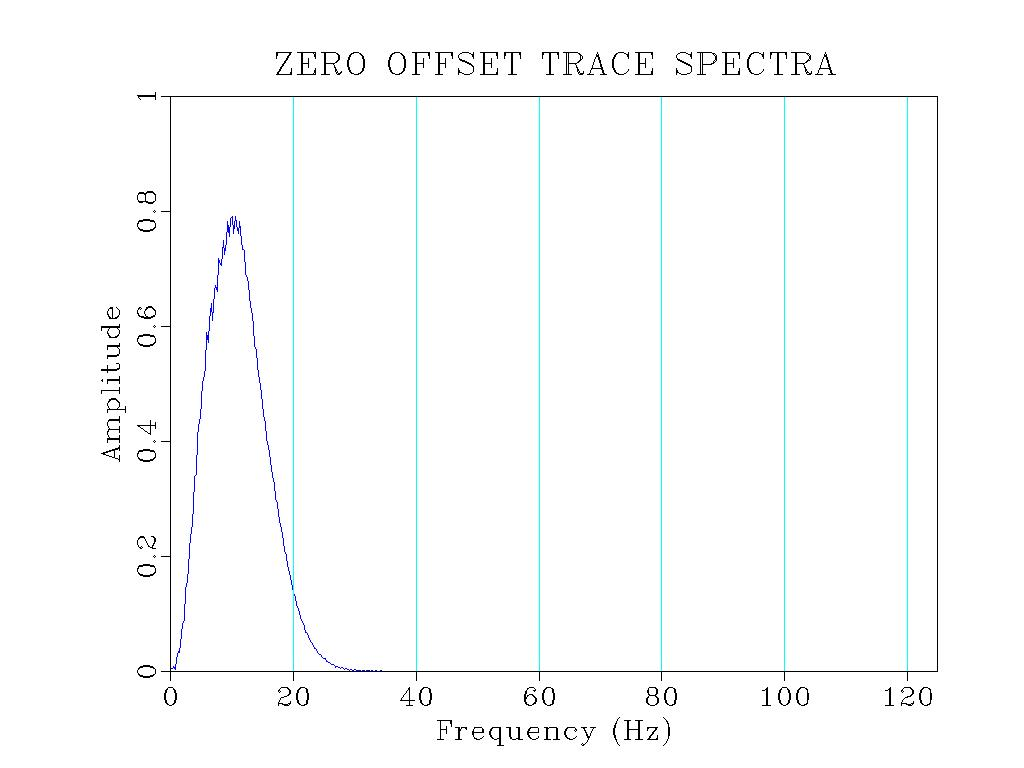
\includegraphics[scale=0.4]{images/originalTraceSpectra.jpeg}
\vspace{-0.3cm}
\end{center}
\begin{center}
 Fonte: Do Autor.
\end{center}
\label{fig:7.1}
\end{figure}


\begin{figure}
\caption{Resultado do empilhamento ERC: Supertraço para m0=4Km. A interpolação e o empilhamento ERC adicionam
ruído numérico aos dados empilhados.}
\begin{center}
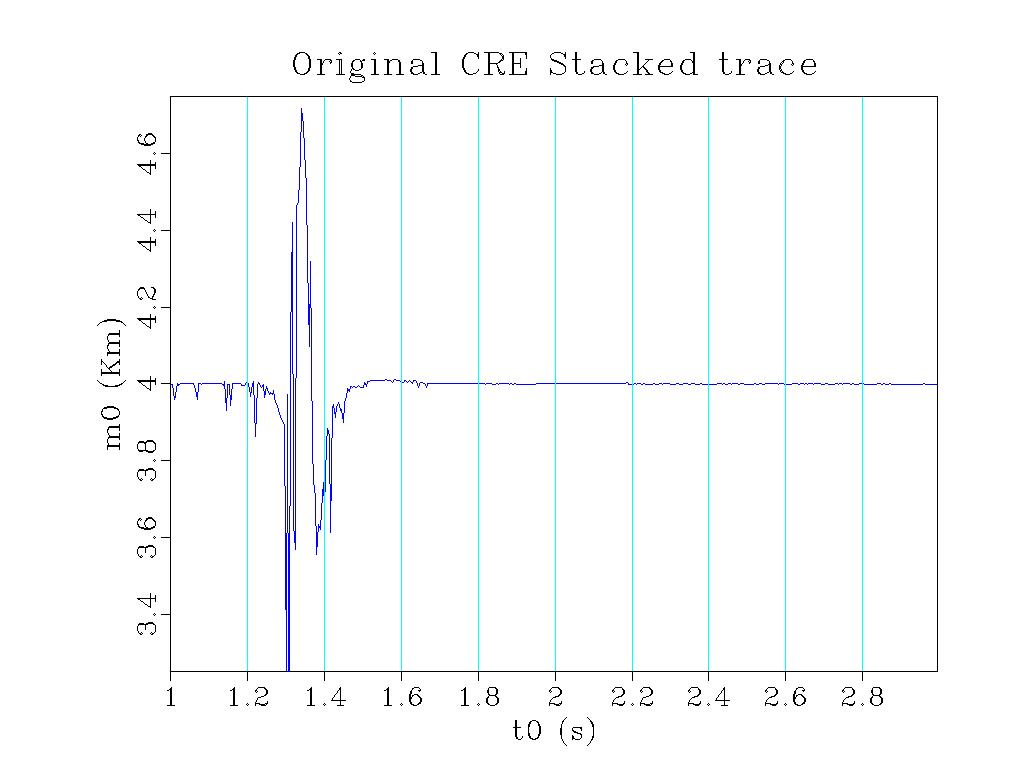
\includegraphics[scale=0.4]{images/creStackedSection.jpeg}
\vspace{-0.3cm}
\end{center}
\begin{center}
 Fonte: Do Autor.
\end{center}
\label{fig:7.2}
\end{figure}

\begin{figure}
\caption{Espectro de amplitude original do supertraço ERC para m0=4Km.}
\begin{center}
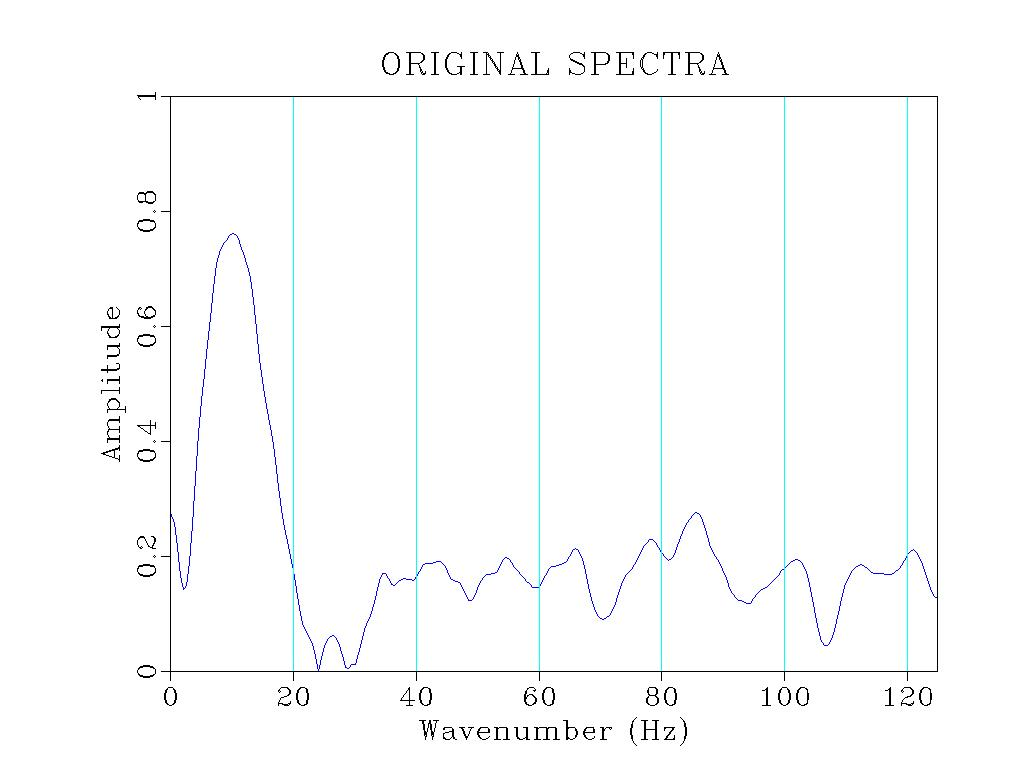
\includegraphics[scale=0.4]{images/originalSpectra.jpeg}
\vspace{-0.3cm}
\end{center}
\begin{center}
 Fonte: Do Autor.
\end{center}
\label{fig:7.3}
\end{figure}

\begin{figure}
\caption{Supertraço ERC após a filtragem banda passante.}
\begin{center}
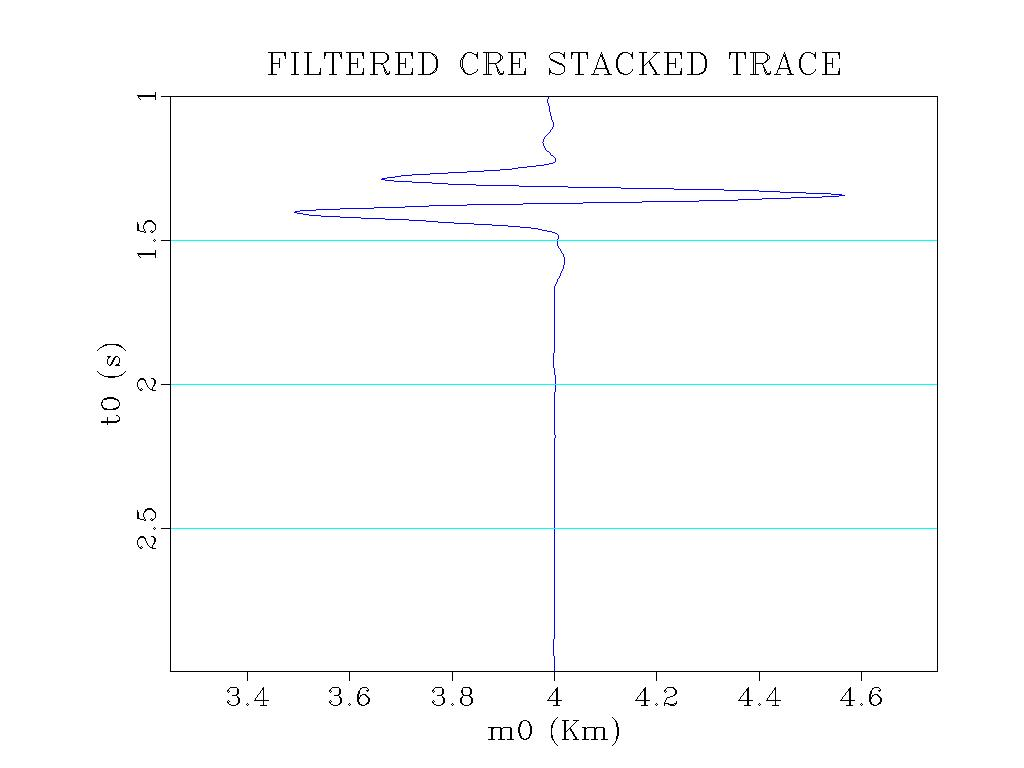
\includegraphics[scale=0.4]{images/creStackedSectionFiltered.jpeg}
\vspace{-0.3cm}
\end{center}
\begin{center}
 Fonte: Do Autor.
\end{center}
\label{fig:7.4}
\end{figure}

\begin{figure}
\caption{Espectro de amplitude após a filtragem banda passante.}
\begin{center}
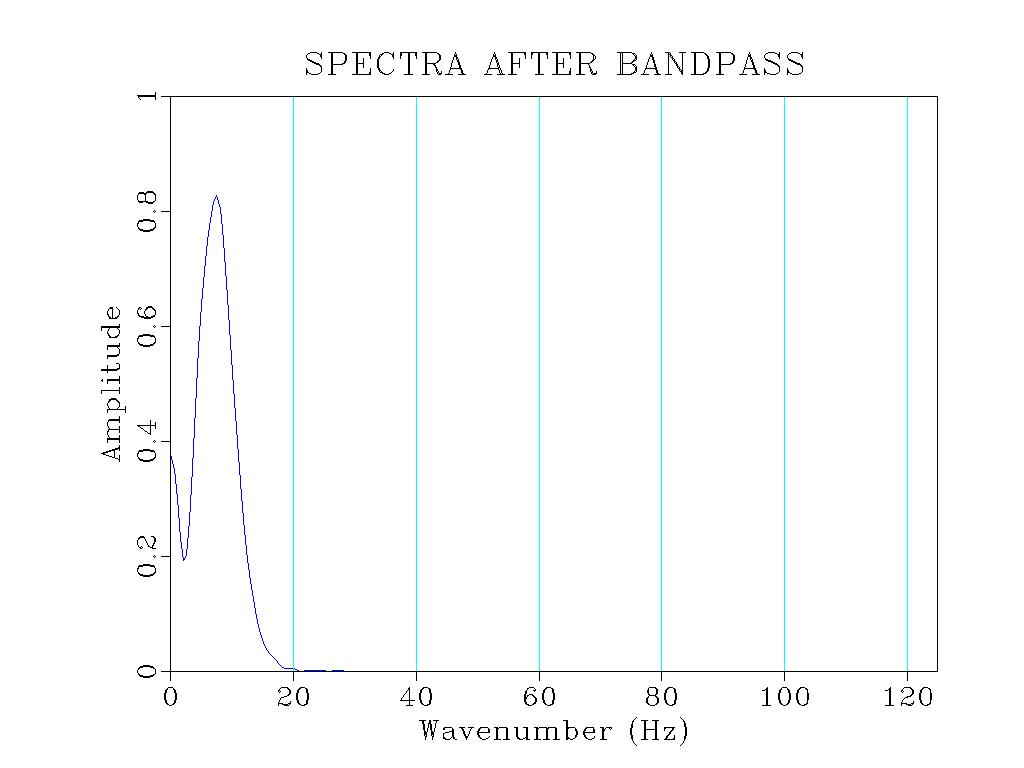
\includegraphics[scale=0.4]{images/filteredSpectra.jpeg}
\vspace{-0.3cm}
\end{center}
\begin{center}
 Fonte: Do Autor.
\end{center}
\label{fig:7.5}
\end{figure}

%% Figuras seção empilhada CRE com a equação de tempo de trânsito CRE

O empilhamento para um dado $m_0$, descrito acima, é realizado para um conjunto de $m_0$'s para formar a seção empilhada.
Cada $m_0$ será um supertraço da seção, como apresentado nas Figuras \ref{fig:7.6}-\ref{fig:7.7} 
que apresentam 4 supertraços empilhados
com $m_0$ variando entre 4Km e 5.5Km com amostragem de 0.5Km.

\begin{figure}
\caption{Supertraços ERC empilhados antes da filtragem banda passante.}
\begin{center}
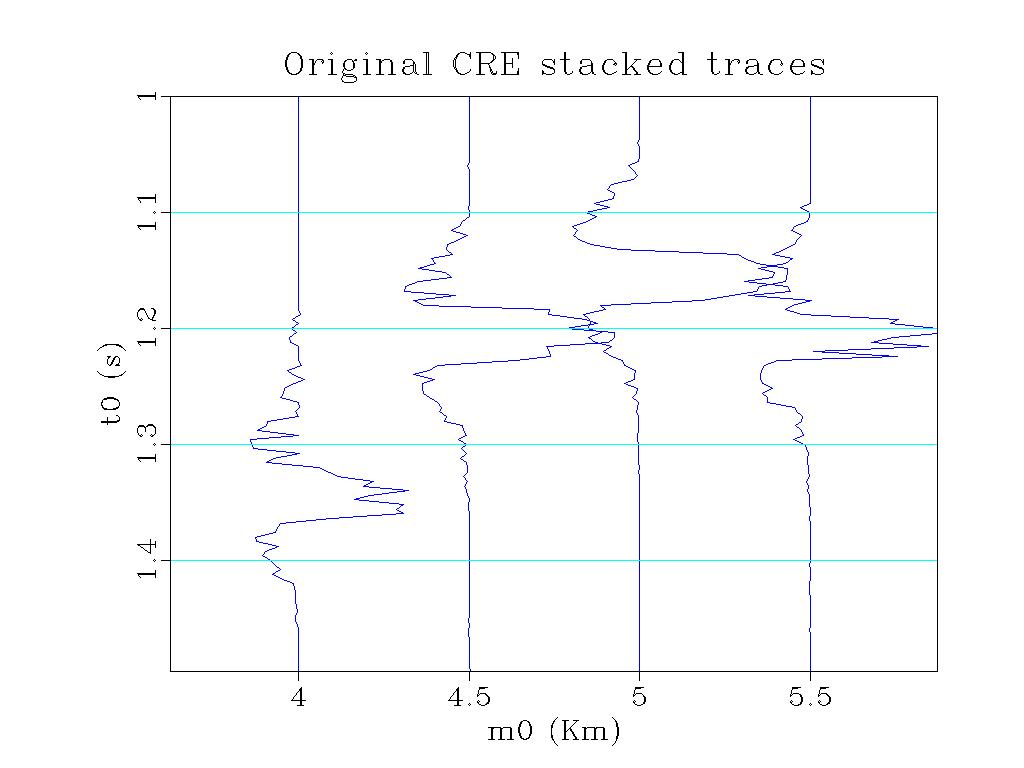
\includegraphics[scale=0.4]{images/stackedTraces.jpeg}
\vspace{-0.3cm}
\end{center}
\begin{center}
 Fonte: Do Autor.
\end{center}
\label{fig:7.6}
\end{figure}

\begin{figure}
\caption{Supertraços ERC empilhados depois da aplicação da filtragem banda passante.}
\begin{center}
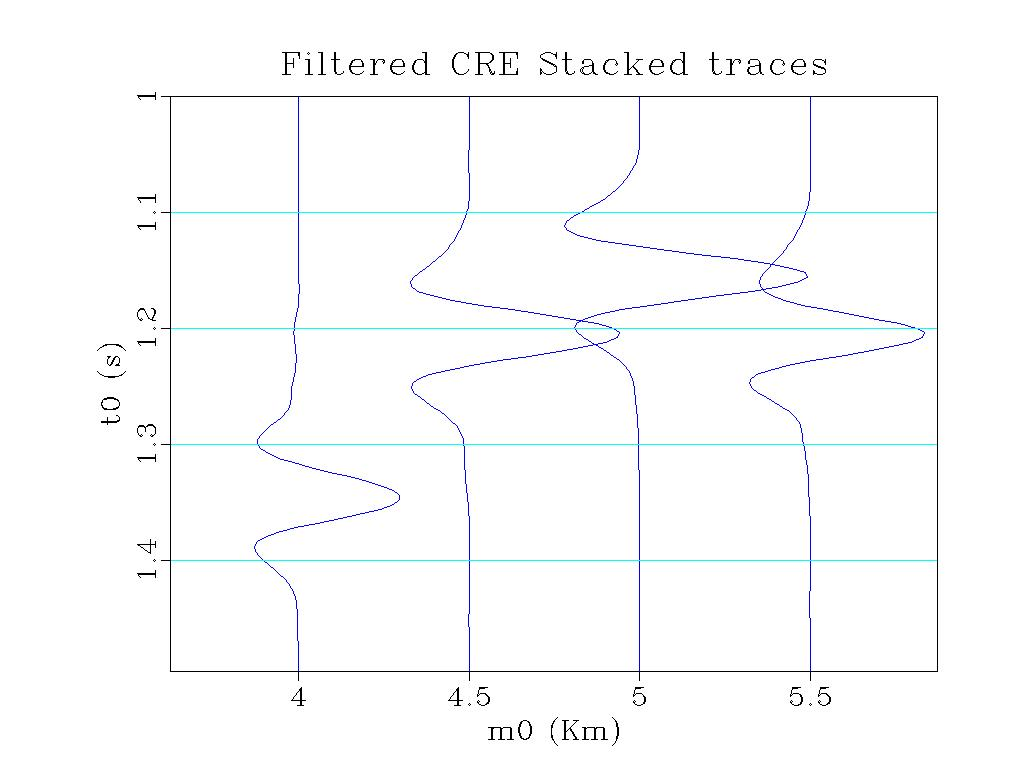
\includegraphics[scale=0.4]{images/filtStackedTraces.jpeg}
\vspace{-0.3cm}
\end{center}
\begin{center}
 Fonte: Do Autor.
\end{center}
\label{fig:7.7}
\end{figure}


Foram produzidas seções empilhadas com 
amostragem entre os PMC's de 0.0125Km, e 160 PMC's no intervalo de $4Km<m<5Km$. O eixo do tempo na 
seção é o tempo de trânsito do raio normal $t_0$ com $1s<t_0<1.5s$, com 125 amostras e amostragem no tempo de 0.004s.
Para comparação dos resultados do empilhamento, foi extraída a seção de afastamento nulo do cubo de dados do modelo do
refletor gaussiano (Figura \ref{fig:4.2} no Capítulo \ref{cap5:modeling}) apresentada na Figura \ref{fig:7.7}.

A Figura \ref{fig:7.8} é o resultado do empilhamento ERC utilizando a aproximação de tempo de trânsito ERC \ref{eq:2.3}
como trajetória de empilhamento. O empilhamento adicionou ruído numérico nos traços da seção, por isto foi realizada a filtragem
banda passante com a frequência máxima de corte em 20Hz. O resultado após a aplicação do filtro é apresentado na Figura
\ref{fig:7.10}.

O empilhamento também foi realizado com auxílio da aproximação de tempo de trânsito SRC não hiperbólica
(Equação \ref{eq:2.4}) aplicando a condição CDS
($R_N=R_{NIP}$). Aplicada esta condição, a curva de tempo de trânsito SRC foi utilizada como trajetória de empilhamento no domínio
ERC, o resultado é apresentado na Figura \ref{fig:7.11}. Também foi realizada a aplicação da filtragem banda passante na seção
empilhada com a aproximação do SRC não hiperbólico, a frequência máxima de corte utilizada foi 20Hz, o resultado é apresentado
na Figura \ref{fig:7.12}.

\begin{figure}
\caption{Seção zero offset extraída do cubo de dados.}
\begin{center}
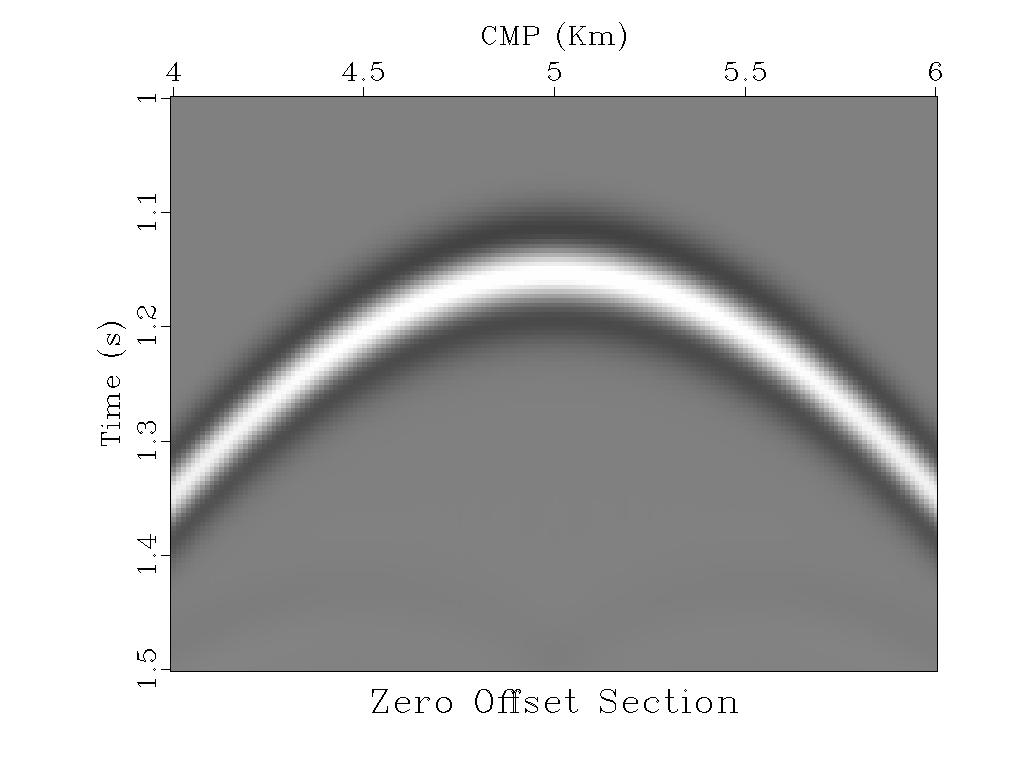
\includegraphics[scale=0.4]{images/zeroOffsetSection.jpeg}
\vspace{-0.3cm}
\end{center}
\begin{center}
 Fonte: Do Autor.
\end{center}
\label{fig:7.8}
\end{figure}

\begin{figure}
\caption{Seção empilhada ERC bruta.}
\begin{center}
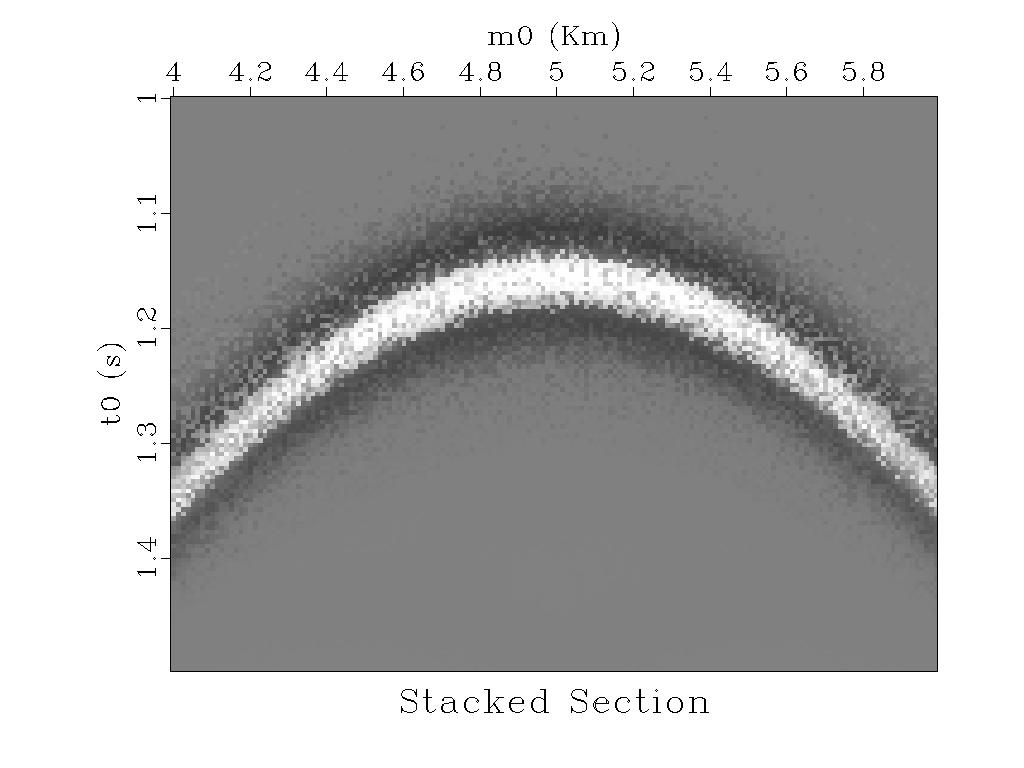
\includegraphics[scale=0.4]{images/stackedSection.jpeg}
\vspace{-0.3cm}
\end{center}
\begin{center}
 Fonte: Do Autor.
\end{center}
\label{fig:7.9}
\end{figure}

\begin{figure}
\caption{Seção empilhada ERC após filtragem de banda passante (Corte em 20Hz).}
\begin{center}
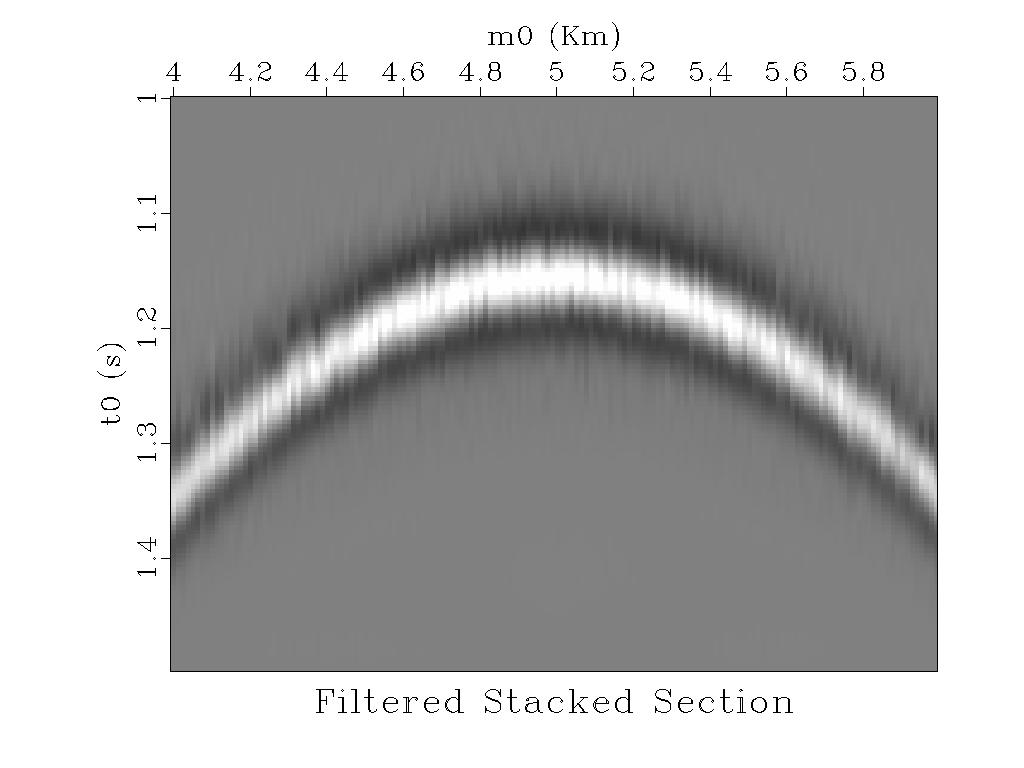
\includegraphics[scale=0.4]{images/filteredStackedSection.jpeg}
\vspace{-0.3cm}
\end{center}
\begin{center}
 Fonte: Do Autor.
\end{center}
\label{fig:7.10}
\end{figure}

%% Figuras Empilhamento CRS não hiperbólico
\begin{figure}
\caption{Seção empilhada ERC bruta produzida a partir do empilhamento sobre a curva de tempo de trânsito SRC não hiperbólica
utilizando a condição CDS ($R_N=R_{NIP}$).}
\begin{center}
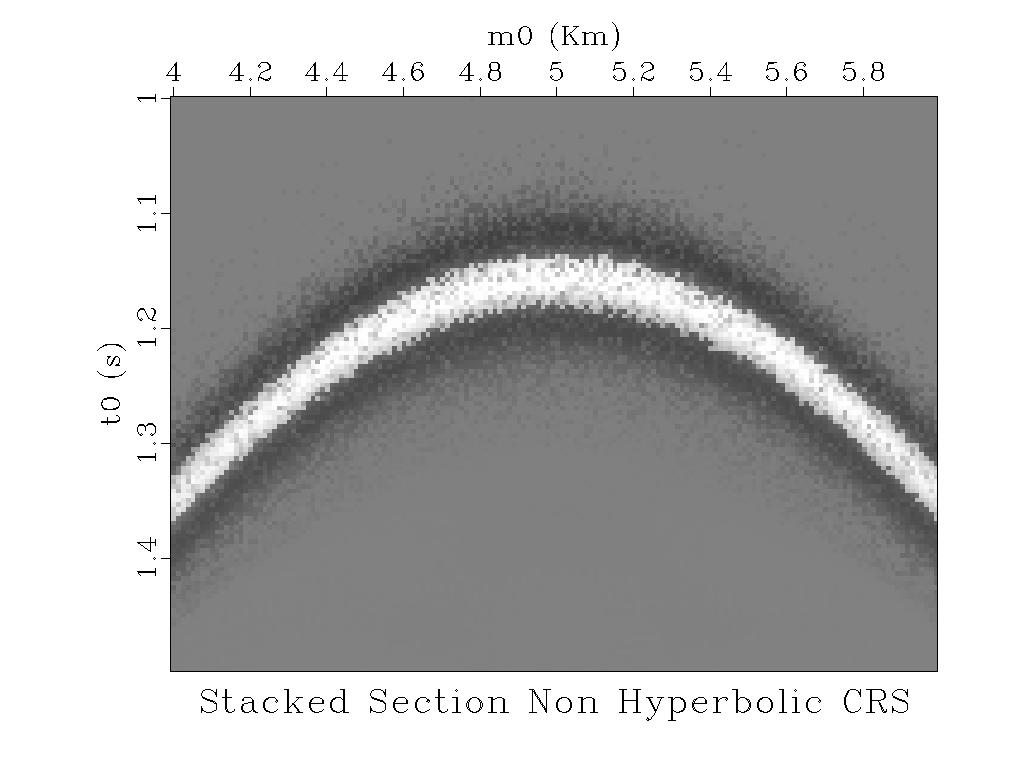
\includegraphics[scale=0.4]{images/stackedSectionNcrs.jpeg}
\vspace{-0.3cm}
\end{center}
\begin{center}
 Fonte: Do Autor.
\end{center}
\label{fig:7.11}
\end{figure}

\begin{figure}
\caption{Seção empilhada ERC após filtragem de banda passante (Corte em 20Hz) produzida a partir do empilhamento 
sobre a curva de tempo de trânsito SRC não hiperbólica
utilizando a condição SDC ($R_N=R_{NIP}$).}
\begin{center}
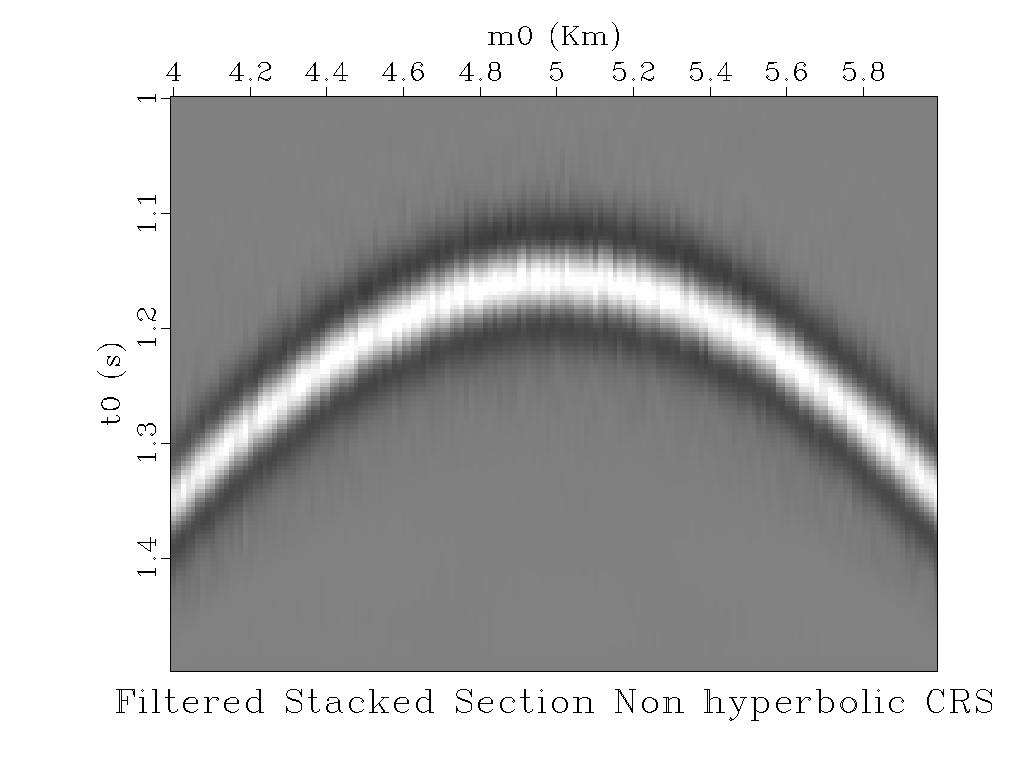
\includegraphics[scale=0.4]{images/filteredStackedSectionNcrs.jpeg}
\vspace{-0.3cm}
\end{center}
\begin{center}
 Fonte: Do Autor.
\end{center}
\label{fig:7.12}
\end{figure}

Refazendo o empilhamento para 320 $m_0$'s separados por 0.0125Km no intervalo
$3Km<m_0<7Km$; e para 500 $t_0$'s no intervalo $1s<t_0<3s$ e amostragem de 0.004s,
obtemos a seção empilhada nas Figuras \ref{fig:7.13}-\ref{fig:7.14}
\footnote{A obtenção das seções empilhadas ERC foi realizada com auxílio de técnicas de computação paralela: Em um computador
de várias CPU's, cada núcleo da CPU é responsável por um $m_0$ (Traço na seção empilhada ERC). O pacote Madagascar permite a
paralelização utilizando a opção \textit{scons -j\#} em que o caractere '\#' representa o número 
de núcleos disponíveis no computador.}.
A aproximação de tempo de trânsito do SRC não hiperbólico aplicada a condição SDC
foi utilizada como trajetória de empilhamento (Equação \ref{eq:2.4}).
A Figura \ref{fig:7.13} é o resultado logo após o empilhamento, e
a Figura \ref{fig:7.14} foi obtida após a aplicação de um filtro banda passante de frequência máxima de corte de 20Hz
na seção empilhada da Figura \ref{fig:7.13}.

%% Figuras Empilhamento CRS não hiperbólico intervalo maior
\begin{figure}
\caption{Seção empilhada ERC bruta produzida a partir do empilhamento sobre a curva de tempo de trânsito SRC não hiperbólica
utilizando a condição CDS ($R_N=R_{NIP}$).}
\begin{center}
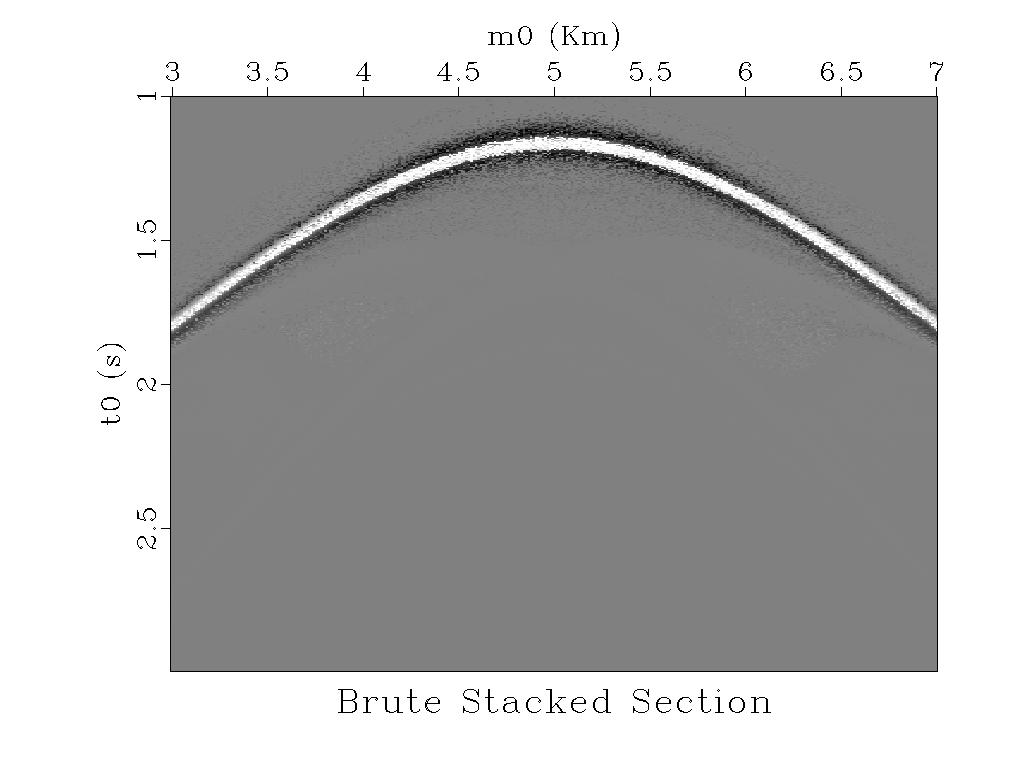
\includegraphics[scale=0.4]{images/hugeStackedSection.jpeg}
\vspace{-0.3cm}
\end{center}
\begin{center}
 Fonte: Do Autor.
\end{center}
\label{fig:7.13}
\end{figure}

\begin{figure}
\caption{Seção empilhada ERC após filtragem de banda passante (Corte em 20Hz) produzida a partir do empilhamento 
sobre a curva de tempo de trânsito SRC não hiperbólica
utilizando a condição SDC ($R_N=R_{NIP}$).}
\begin{center}
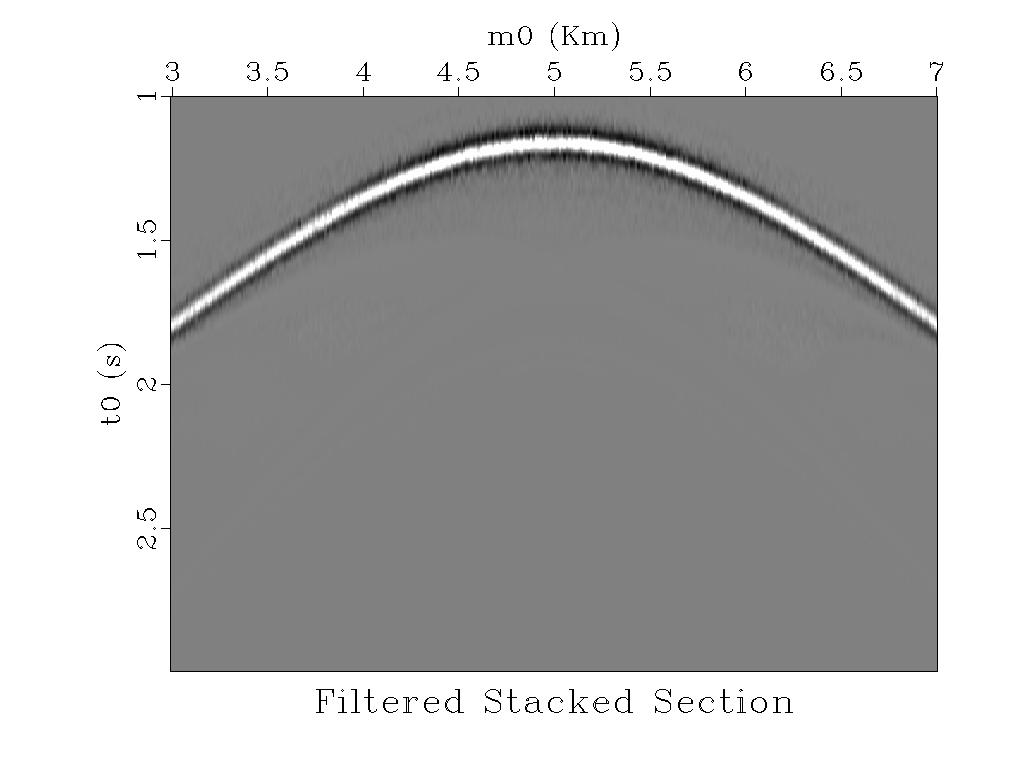
\includegraphics[scale=0.4]{images/hugeFiltStackedSection.jpeg}
\vspace{-0.3cm}
\end{center}
\begin{center}
 Fonte: Do Autor.
\end{center}
\label{fig:7.14}
\end{figure}